%TODO: add cliffhanger with preview for next time

% Make nice A4 pages for print:
%\usepackage{pgfpages}
%\pgfpagesuselayout{resize to}[a4paper,border shrink=5mm,landscape]

\beamertemplatenavigationsymbolsempty

\setbeamertemplate{bibliography item}[text]

\usepackage[type={CC},modifier={by-sa},version={4.0}]{doclicense}

\usepackage[utf8]{inputenc}
\usepackage{hyperref}
\usepackage{breakurl}
\usepackage{graphicx}
\usepackage{pgfplots}
\usepackage{pgf}
\usepackage{tikz}
\usetikzlibrary{positioning}
\usetikzlibrary{arrows}
\usetikzlibrary{decorations.markings}
\usetikzlibrary{calc}
\usetikzlibrary{matrix}
\usetikzlibrary{shapes}
\usetikzlibrary{decorations.pathmorphing}
\usetikzlibrary{fit}
\usetikzlibrary{backgrounds}
\usetikzlibrary{plotmarks}
\usepackage{stmaryrd}
\usepackage{listings}
\usepackage{pdflscape}
\usepackage{perpage}
\usepackage{appendixnumberbeamer}

%\usepackage[thmmarks,amsmath,amsthm]{ntheorem} % already included in beamer
\usepackage{thm-restate}

\usepackage[sort&compress,numbers]{natbib}  % to be have \citet, \citeauthor, \citeyear

\MakePerPage{footnote}

\tikzstyle{o}=[r,ppBlue]
\tikzstyle{r}=[thick,rectangle,align=center]
\tikzstyle{t}=[r,ppTrans] %,font=\bfseries]
\tikzstyle{dd}=[densely dashed]
\tikzstyle{n}=[r,ppBlue]
\tikzstyle{p}=[r,ppRed]
\tikzstyle{ppRed}  =[draw=red,  fill=  red!20]
\tikzstyle{ppBlue} =[draw=blue, fill= blue!20]
\tikzstyle{ppGreen}=[draw=green,fill=green!20]
\tikzstyle{ppTrans}=[draw=none, fill=none]

\usetheme{Warsaw}

\useoutertheme[subsection=true]{smoothbars}
%\useoutertheme[subsection=false]{miniframes}

\definecolor{bblue}{HTML}{D7DF01}	% yellow-ish actually, for better black/white printing
\definecolor{rred}{HTML}{C0504D}
\definecolor{ggreen}{HTML}{9BBB59}
\definecolor{ppurple}{HTML}{9F4C7C}
\definecolor{lightgray}{rgb}{0.3,0.3,0.3}
\definecolor{lightergray}{rgb}{0.9,0.9,0.9}
\definecolor{UniBlue}{RGB}{83,121,170}

\DeclareTextFontCommand\textintro{\normalfont\bfseries\itshape} % nice!
\newcommand{\intro}[2][]
{%
	\textintro{#2}%
}
\newcommand{\empha}[2][]
{%
	\emph{#2}%
}

%\theoremstyle{plain}
\newcounter{reqcounter}
\newtheorem{requirement}[reqcounter]{Requirement}

%setbeamercolor{structure}{fg=violet}

\makeatletter
\def\th@task{%
    \normalfont % body font
    \setbeamercolor{block title example}{bg=orange,fg=white}
    \setbeamercolor{block body example}{bg=orange!20,fg=black}
    \def\inserttheoremblockenv{exampleblock}
  }
\makeatother

\theoremstyle{task}
\newtheorem{task}{Task}

\newenvironment{assignment}%
{%\setbeamercolor{background canvas}{bg=violet}%
%\setbeamercolor{structure}{fg=cyan!90!black}%
 \setbeamercolor{frametitle}{bg=orange,fg=white}
\begin{frame}}%
{\end{frame}}%

\AtBeginSection[]{
  \begin{frame}
  \vfill
  \centering
  \begin{beamercolorbox}[sep=8pt,center,shadow=true,rounded=true]{title}
    \usebeamerfont{title}\insertsectionhead\par%
  \end{beamercolorbox}
  \tableofcontents
  \vfill
  \end{frame}
}




\pgfplotsset{compat=1.14}
\author{Markus Raab}


\date{27.3.2019}

\begin{document}

\renewcommand{\enquote}[1]{\emph{``#1''}} % Cannot be done earlier

%%%%%%%%%%%%%%%%%%%%%%%%%%%%%%%
\begin{frame}
	\titlepage
	\doclicenseThis
\end{frame}

\begin{frame}
	Lecture is every week Wednesday 09:00 - 11:00.

	\begin{description}
		\item[06.03.2019:] {\color{gray}topic, teams}
		\item[13.03.2019:] {\color{gray}TISS registration, initial PR}
		\item[20.03.2019:] {\color{gray}other registrations, guest lecture}
		\item[27.03.2019:] {\color{red}PR for first issue done, second started, \\ HS: kleiner Schiffbau}
		\item[03.04.2019:] {\color{orange}first issue done, PR for second}
		\item[10.04.2019:] mid-term submission of exercises
		\item[08.05.2019:] (HS?)
		\item[15.05.2019:]
		\item[22.05.2019:]
		\item[29.05.2019:]
		\item[05.06.2019:] final submission of exercises
		\item[12.06.2019:]
		\item[19.06.2019:] last corrections of exercises
		\item[26.06.2019:] exam
	\end{description}
\end{frame}

\begin{frame}
	\frametitle{Popular Topics}
	\vspace{-0.55cm}
	\setlength{\columnsep}{-1.3cm}
	\raggedright
	\begin{multicols}{2}
	\begin{description}
	\item[14] tools
	\item[9] testability
	\item[9] code-generation
	\item[7] context-awareness
	\item[6] {\color{orange} specification}
	\item[6] misconfiguration
	\item[6] {\color{red} complexity reduction}
	\item[5] validation
	\item[5] points in time % (early detection)
	\item[5] error messages
	\item[5] auto-detection
	\item[4] user interface
	\item[4] introspection
	\item[4] design
	\item[4] cascading
	\item[4] architecture of access
	\item[3] {\color{red} configuration sources}
	\item[3] {\color{orange} config-less systems}
	\item[2] secure conf
	\item[2] {\color{orange} architectural decisions}
	\item[1] push vs.\ pull
	\item[1] infrastructure as code
	\item[1] full vs.\ partial
	\item[1] convention over conf %iguration
	\item[1] CI/CD
	\item[0] documentation
	\end{description}
	\end{multicols}
\end{frame}

\begin{assignment}
	\frametitle{Tasks for today}
	(until 27.03.2019 23:59)

	\begin{task}
	Description of homework as pull request in private repo.
	(Inside a folder for you, use GitHub name.)
	\end{task}

	\begin{task}
	Description of teamwork (which application, which CM tool) as pull request in private repo.
	(Inside a folder for your team.)
	\end{task}

	\begin{task}
	Fix at least one issue and write some text in at least one other issue.
	\end{task}
\end{assignment}

\begin{frame}
	\frametitle{Slides}
	\begin{itemize}
	\item slide numbering: 02a is after 02
	\item old slides in same repo: always check date
	\end{itemize}
\end{frame}

\begin{frame}
	\frametitle{Some misconfigurations}
	\begin{itemize}
	\item studycode is Studienkennzahl
	\item same name twice in TALKS.xml
	\item \dots
	\end{itemize}

	\begin{task}
	How did these misconfigurations happened?
	\end{task}
\end{frame}

\begin{assignment}
	\frametitle{Tasks for next week}
	(until 03.04.2019 23:59)

	\begin{task}
	Fix misconfigurations in private repo.
	\end{task}

	\begin{task}
	Fix feedback about homework/teamwork.
	Calculate complexity of your teamwork.
	\end{task}

	\begin{task}
	First issue done, PR for second issue and write some text in at least one other issue (if 5 issues are not yet assigned to you).
	\end{task}
\end{assignment}


\begin{frame}
	\frametitle{KeySet (Recapitulation)}

	The common data structure between plugins:
	\vspace{1cm}

	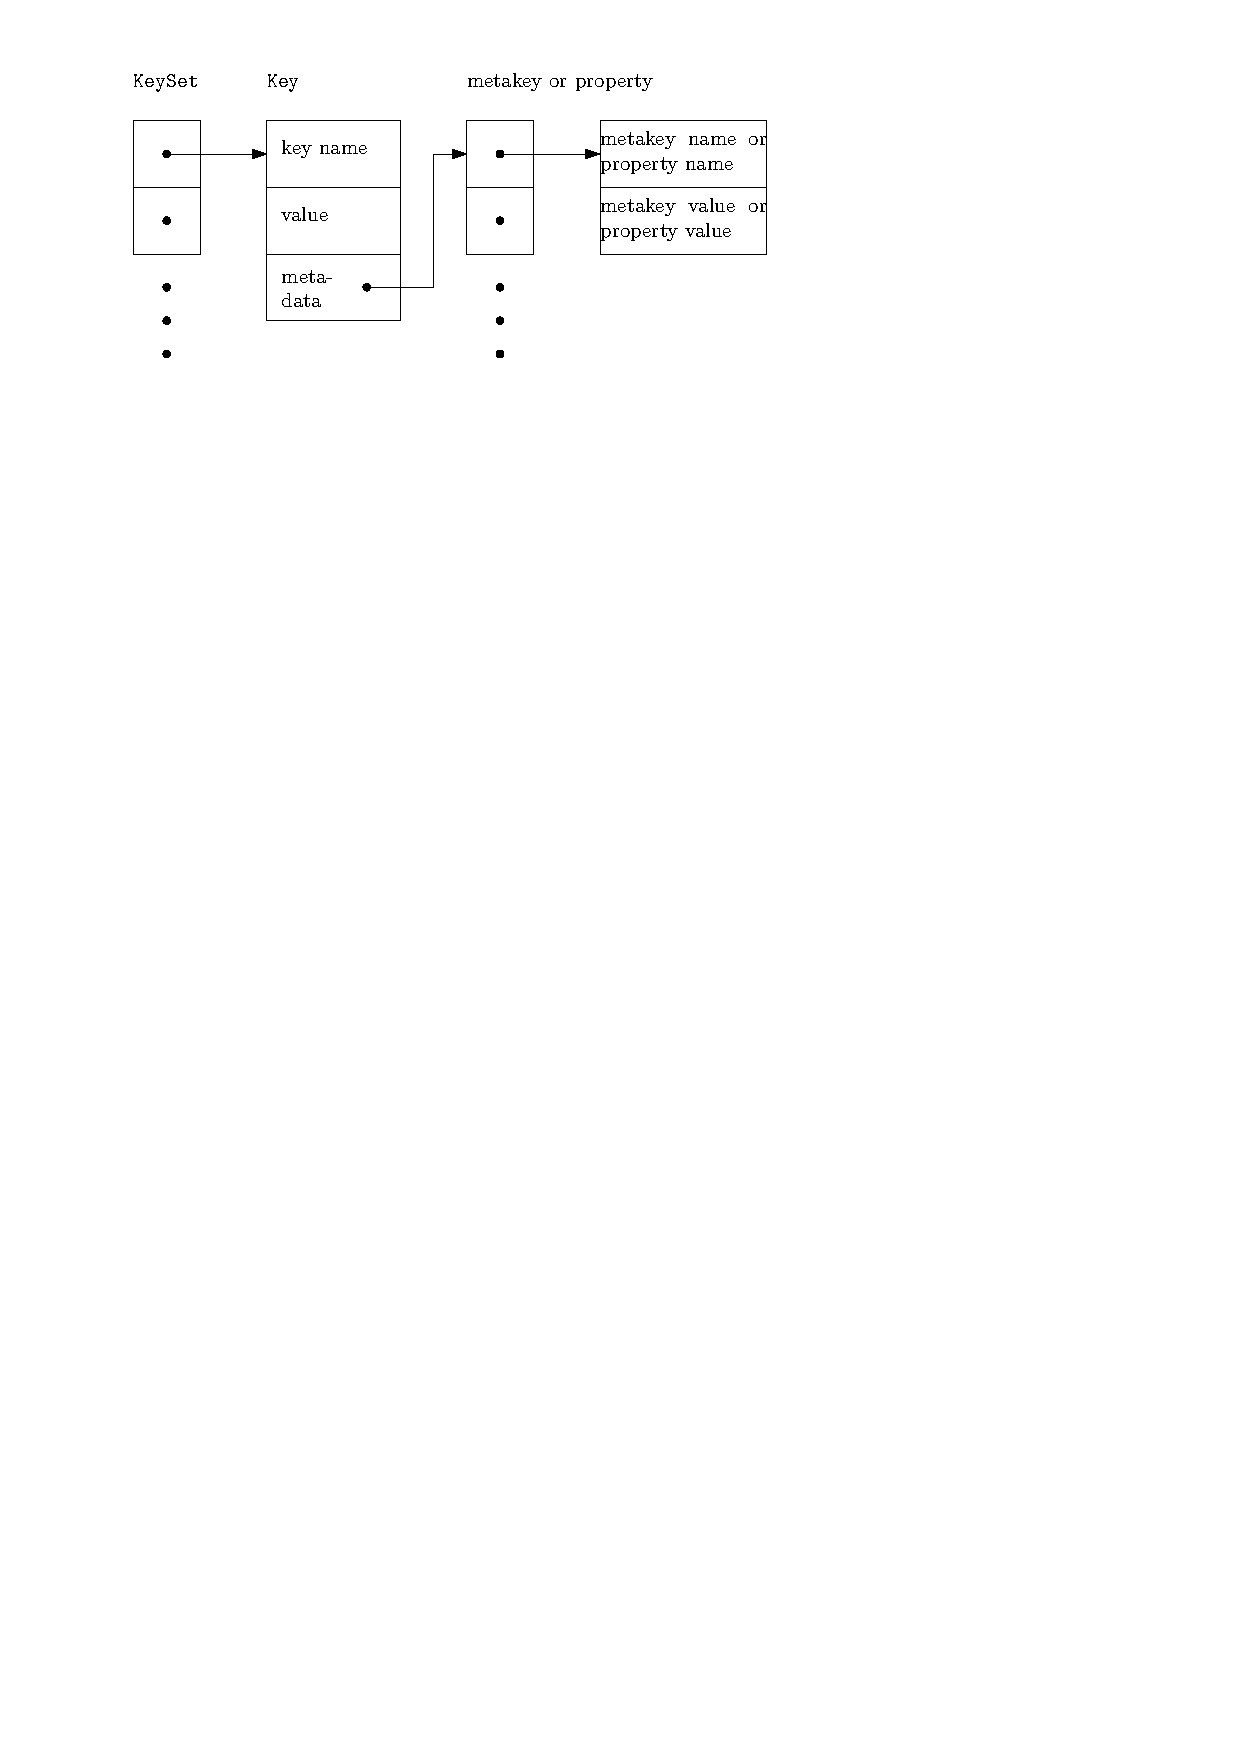
\includegraphics{keyset}
\end{frame}

\begin{frame}
	\frametitle{Recapitulation}

	\methodQuestion{} \question{Which configuration systems/libraries/APIs have you already used or would like to use in one of your FLOSS project(s)?}
	\pause
	\begin{itemize}
	\item command-line arguments (\p{92}, $n=222$)
	\item environment variables (\p{79}, $n=218$)
	\item configuration files (\p{74}, $n=218$))
	\end{itemize}
\end{frame}

\begin{frame}
	\frametitle{Semantics of Command-line Arguments (cont.)}
	\begin{itemize}
	\item passed by main for a new process via \\ (\texttt{int argc, char ** argv})
	\item visible from other processes (e.g., via \texttt{ps aux})
	\item could be passed along to subprocesses but hardly done
	\item need to be parsed by process
	\item portability: differences in parsing
	\item cannot be changed from outside (requires restart, no IPC)
	\end{itemize}
\end{frame}

\begin{frame}
	\frametitle{Talk}
	Miruna Orsa

	Using XML in the day to day work life
\end{frame}



%%%%%%%%%%%%%%%%%%%%%%%%%%%%%%%%%%%%%%%%%% 
\section{Environment Variables}

\begin{frame}
	\frametitle{Semantics}
	\begin{itemize}
	\item are also per-process (\texttt{/proc/self/environ})
	\item are not visible from other processes
	\item are automatically inherited by subprocesses
	\item need to be parsed by process (\texttt{[extern] char **environ}) but API is provided (\texttt{getenv})
	\item cannot be changed from outside (requires restart or an additional IPC mechanism)
	\end{itemize}
\end{frame}

\begin{frame}
	\frametitle{getenv}
	\begin{itemize}
	\item is widely standardized, including SVr4, POSIX.1-2001, 4.3BSD, C89, C99~\cite{man2017getenv},
	\item is supported by many programming languages, and
	\item enforces \texttt{key=value} convention.
	\end{itemize}
\end{frame}

\begin{frame}
	\frametitle{Usage}
	\begin{enumerate}
	\item bypassing other configuration accesses (\methodQuestion{} \p{45})
	\item locating configuration files
	\item debugging and testing (\methodQuestion{} \p{55}, \methodSource{} 1,152, i.\,e. \p{43})
	\item sharing configuration settings across applications (\methodQuestion{} \p{53}, \methodSource{} 716, i.\,e. \p{47})
	\item for configuration settings unlikely to be changed by a user (\methodQuestion{} \p{20})
	\item \question{even when it is used inside a loop} (\methodQuestion{} \p{2})
	\end{enumerate}
\end{frame}

\begin{frame}
	\frametitle{Portability}
	\begin{itemize}
	\item no separators for values defined
	\item case sensitivity problems
	\item often many environment variables for the same purpose: TMP, TEMP, or TMPDIR
	\item sometimes one environment variable for different purposes: PATH
	\end{itemize}
\end{frame}

\begin{assignment}
	\begin{task}
	What is wrong with the code in the book?
	\end{task}
\end{assignment}



\subsection{Requirements}

\begin{frame}
	How can we deal with the many sources?

	\vspace{1cm}

	\begin{restatable}{requirement}{reqEnvironment}
	A configuration library must support all three popular ways for configuration access:
	configuration files, command-line options, and environment variables.
	\end{restatable}
\end{frame}

\begin{frame}[fragile]
	\frametitle{Example: Elektra}

	\begin{itemize}
	\item includes library libopts
	\item which provides the function ^int elektraGetOpts (KeySet, argc, argv, environ, Key)^
	\item which puts ^Key^s in the ^proc^ namespace
	\item \url{https://www.libelektra.org/tutorials/command-line-options}
	\end{itemize}

	\pause
	\vspace{1cm}

	What is a namespace?
\end{frame}

\begin{frame}
	\frametitle{Cascading}
	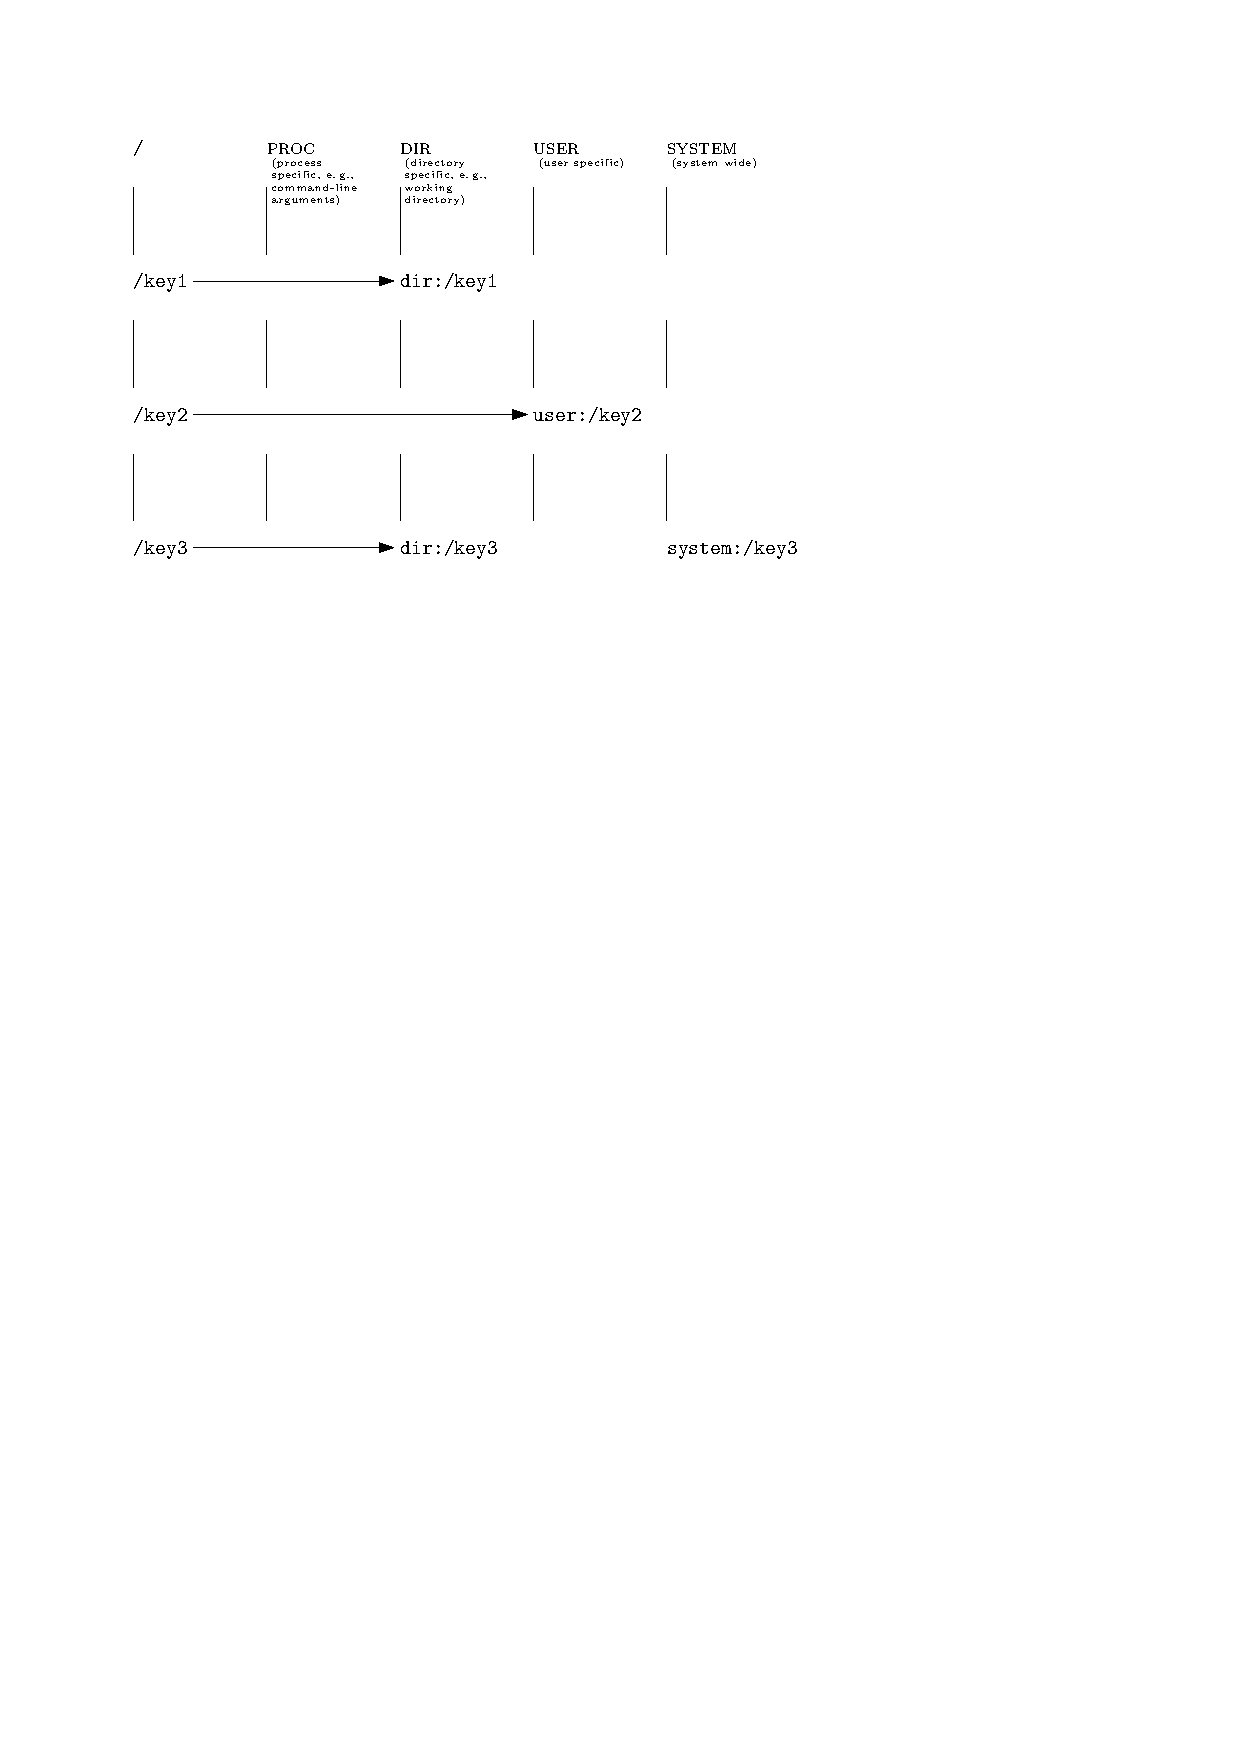
\includegraphics{cascading}
\end{frame}

\begin{assignment}
	\begin{task}
	Discuss the differences of mounting and cascading with your neighbor.
	\end{task}
\end{assignment}


\subsection{Conclusion}

\begin{frame}
	\frametitle{User View}
	\begin{itemize}
	\item command-line for trying out configuration settings
	\item environment variables for configuration settings within a shell
	\item configuration files for persistent configuration settings
	\end{itemize}
\end{frame}

\begin{frame}
	\frametitle{Conclusion}
	\begin{itemize}
	\item three different configuration sources widely used
	\item all three used for different reasons but often for the same configuration settings
	\item many different configuration file formats
	\item abstractions: key-value, mounting, and cascading
	\end{itemize}
\end{frame}






%%%%%%%%%%%%%%%%%%%%%%%%%%%%%%%%%%%%%%%%%% 
\section{Complexity}

\subsection{Trend}

\begin{frame}
	\frametitle{Trend Firefox}
	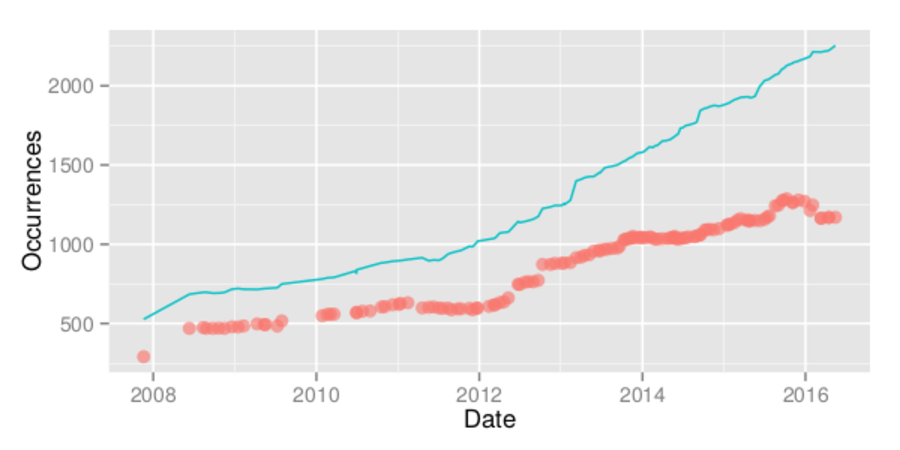
\includegraphics[scale=0.7]{firefox}
\end{frame}

\begin{frame}
	\frametitle{Trend Chromium}
	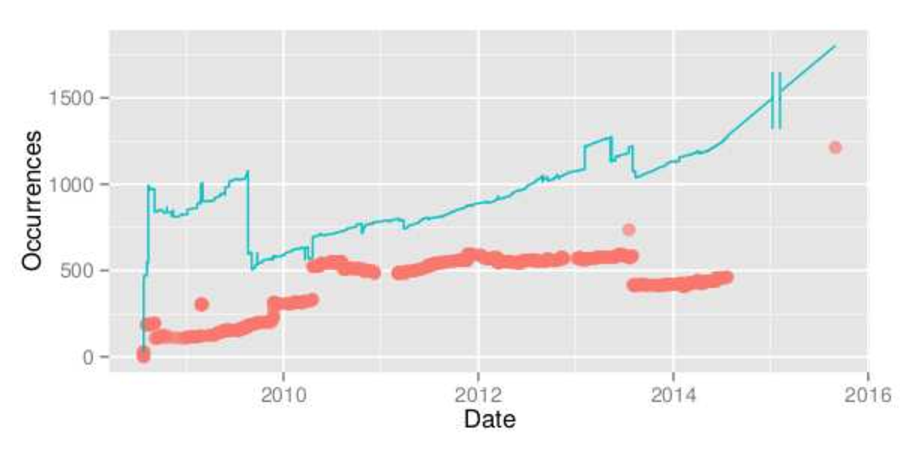
\includegraphics[scale=0.7]{chromium}
\end{frame}

\begin{frame}
	\frametitle{Trend Configuration Files}
	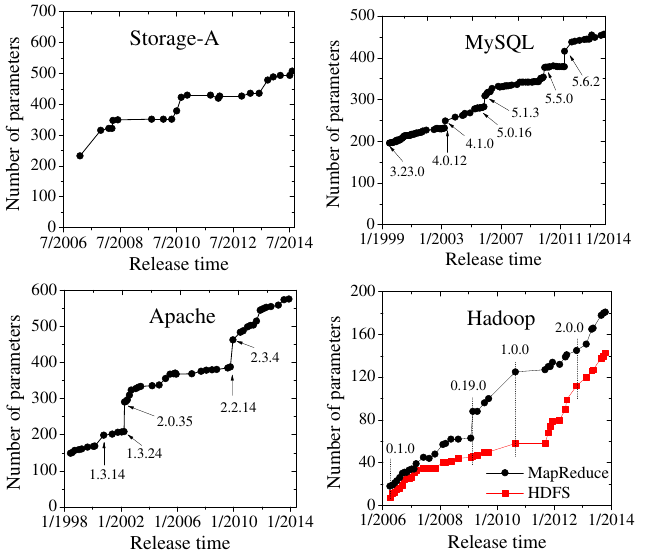
\includegraphics[scale=0.5]{pics/trend.png}
	\citet{xu2015hey}
\end{frame}

\subsection{Calculation}

\begin{frame}
	\frametitle{Types of Complexity}
	\begin{itemize}
	\item complexity in access:
		\begin{itemize}
		\item many different formats
		\item non-uniformity
		\item transformations
		\end{itemize}
	\item configuration settings
		\begin{itemize}
		\item number of settings $s$
		\item number of values $n$
		\item dependences between settings
		\end{itemize}
	\end{itemize}
\end{frame}

\lstDeleteShortInline^
\begin{frame}
	\frametitle{Calculation of Complexity}

	Using enumerative combinatorics:
	\begin{itemize}
	\item number of configurations: $n^s$
	\item for $N$ groups of different $n$ and $s$ (i.e., $n_1 \dots n_N$ with $s_1 \dots s_N$ occurrences):  $$\prod_{i=1}^{N} n_i^{s_i}$$
	\item more difficult to calculate (or unbounded) for dependences, module instantiations, arrays, \dots
	\end{itemize}
\end{frame}

\begin{frame}
	\frametitle{Calculation of Complexity}

	Examples:
	\begin{itemize}
	\item 600 boolean settings in Apache httpd (let us assume $n=2$):
	\pause
	$2^{600} \approx 10^{180}$

	\item 19 integer settings:
	\pause
	${2^{32}}^{19} = 2^{32 \cdot 19} = 2^{609} \approx 10^{183}$

	\item 2000 boolean settings in Firefox~\cite{jin2014configurations}:
	\pause
	$2^{2000} \approx 10^{602}$
	\end{itemize}
\end{frame}

\begin{assignment}
	\begin{task}
	Break.
	\end{task}
\end{assignment}

%TODO: Firefox and LibreOffice is known, see calculation in jin2014configurations (RQ 1)

\begin{frame}
	\frametitle{Calculation of Complexity (cont.)}

	Examples:
	\begin{itemize}
	\item for 20 boolean and 20 enums with 5 possibilities:
	\pause
	$$2^{20}*5^{20} = 10^{20}$$

	\item MySQL has 461 settings, of which 216 are non-simple types~\cite{xu2015hey} \\ (let us assume $n=\{3,20\}$):
	\pause
	$3^{245} * 20^{216} \approx 10^{397}$ \\
	(settings are explained in 5560 pages\footnote{\url{https://downloads.mysql.com/docs/refman-5.7-en.pdf}})

	\item an array with $1-20$ boolean settings:
	\pause
	$2^{20}$
	\end{itemize}
\end{frame}
\lstMakeShortInline[postbreak=,keywordstyle={},showspaces=no]^
%XXX

\begin{assignment}
	\begin{task}
	Calculate complexity of your teamwork and add to PR.
	\end{task}

	See scripts/complexity.rb
\end{assignment}

\begin{frame}
	\frametitle{Decision Tree}
	\begin{itemize}
	\item configuration settings may depend on each other
	\item form a decision tree~\cite{reiser2009cvm,czarnecki2012cool}
	\item the decision tree is an instantiation of chosen configuration settings
	\item calculation only needs to consider instantiations which make a difference: \\
	essential configuration complexity~\cite{meinicke2016essential}
	\end{itemize}
\end{frame}

\subsection{Usage}

\begin{frame}[fragile]
	\frametitle{Harmful Defaults~\cite{xu2015hey}}
	\begin{itemize}
	\item Problem: Two major data losses on a dozen machines.
	\item Cause:
	Stayed with the default values of the data-path settings
	(e.g., ^dfs.name.dir^, ^dfs.data.dir^) which point to locations in ^/tmp^.
	Thus, after the machines reboot, data losses occur.
	``One of the common problems from users.'' (from Cloudera)
	\item up to \p{53} of misconfigurations is due to staying at defaults
	\item \p{17} to \p{48} of configuration issues are about difficulties in finding settings
	\end{itemize}
\end{frame}

\begin{frame}[fragile]
	\frametitle{Unnecessary Settings~\cite{xu2015hey}}
	\begin{itemize}
	\item Configuration Parameter: ^dfs.namenode.tolerate.heartbeat.multiplier^
	\item Developers' Discussion:
	Since we are not sure what is a good choice, how about making it
	configurable?
	We should add a configuration option for it. Even if it's unlikely to
	change, if someone does want to change it they'll thank us that they
	don't have to change the code/recompile to do so.
	\item Real-World Usage:
	\begin{itemize}
	\item No usage found by searching the entire mailing lists and Google.
	\item No usage reported in a survey of 15 Hadoop users in UCSD.
	\end{itemize}
	\end{itemize}
\end{frame}

\begin{frame}
	\frametitle{Unnecessary Settings~\cite{xu2015hey}}
	\begin{itemize}
	\item \p{6} to \p{17} of settings set by majority
	\item up to \p{54} are seldom set
	\item up to \p{47} of numeric settings have no more than five distinct values
	\end{itemize}
\end{frame}

\begin{frame}
	\frametitle{Reduction}
	\methodQuestion{}
	\question{Why do you think configuration should be reduced?}
	\begin{itemize}
	\item to simplify code maintenance (\p{50}),
	\item to prevent errors and misconfiguration (\p{43}),
	\item to provide better user experience (\p{40}),
	\item \textbf{\question{I do not think it should be reduced} (\p{30})},
	\item because they prefer auto-detection (\p{29}) \\ (with a possibility to override configuration settings: \p{32}),
	\item \question{because use-cases which are rarely used should not be supported} (\p{13}),
	\item \question{never find time for this task} (\p{9}), and
	\item \question{because only standard use-cases should be supported} (\p{1})
	\end{itemize}
\end{frame}

\begin{frame}
	\begin{alertblock}{Question}
	How to specify reduction strategies of configuration settings?
	\end{alertblock}
	\pause
	\begin{exampleblock}{Answer}
	Configuration Specification
	\end{exampleblock}
\end{frame}



%%%%%%%%%%%%%%%%%%%%%%%%%%%%%%%%%%%%%%%%%% 
\section{Configuration Specification}

\subsection{Why?}

\begin{frame}
	\frametitle{Rationale}
	\begin{itemize}
	\item without specification you and others do not even know which settings are available
	\item needed for any further techniques we will discuss
	\pause
	\item essential for \intro[no-futz computing]{no-futz computing}~\citet{holland2001nofutz}
	\item the foundation for any advanced tooling like configuration management tools
	\pause
	\item needed as communication of producers and consumers of configuration
	\end{itemize}
\end{frame}


%%%%%%%%%%%%%%%%%%%%%%%%%%%%%%%%%%%%%%%%%% 
\nocite{raab2017introducing}

\appendix

\begin{frame}[allowframebreaks]
	\bibliographystyle{plainnat}
	\bibliography{../shared/elektra.bib}
\end{frame}

\end{document}


